\documentclass[11pt,a4paper]{article}
\usepackage[margin=0.85in]{geometry}
\usepackage[T1]{fontenc}
\usepackage{lmodern}
\usepackage{amsmath,amssymb,mathtools}
\usepackage{graphicx,booktabs,array,enumitem}
\usepackage[dvipsnames]{xcolor}
\usepackage{microtype}
\usepackage{caption}
\usepackage{listings}
\usepackage{hyperref}
\hypersetup{colorlinks=true,linkcolor=MidnightBlue,urlcolor=MidnightBlue,
  pdfauthor={},pdfsubject={Reinforcement learning worked solutions}}
\setlength{\parindent}{0pt}
\setlength{\parskip}{6pt}
\setlist{nosep,leftmargin=*}
\setlength{\emergencystretch}{2em}
\captionsetup{font=small,labelfont=bf}
\lstset{basicstyle=\ttfamily\small,breaklines=true,
  columns=fullflexible,keepspaces=true,showstringspaces=false,
  commentstyle=\color{gray},keywordstyle=\color{MidnightBlue},
  aboveskip=6pt,belowskip=6pt}
\newcommand{\E}{\mathbb{E}}
\newcommand{\R}{\mathbb{R}}
\newcommand{\norm}[1]{\left\lVert #1\right\rVert}
\newcommand{\sg}{\operatorname{stopgrad}}
\DeclareMathOperator*{\argmax}{arg\,max}
\DeclareMathOperator*{\argmin}{arg\,min}
\newcommand{\studytitle}[1]{%
  \hypersetup{pdftitle={#1 - Worked Solutions}}%
  {\small\color{MidnightBlue} BASICRL\quad /\quad WORKED SOLUTIONS}\par
  \vspace{5pt}{\LARGE\bfseries #1}\par\vspace{5pt}}
\newcommand{\historical}{\textbf{Experiment status.} The following numbers and
  curves are retained from earlier runs, not from a rerun of the revised
  reference code. They are examples for interpretation, not performance guarantees.\par}

\begin{document}
\studytitle{Visual State Estimation and Control}

\section{Aligning images with state targets}
Collect a rendered image $I_t$ and its corresponding state $s_t$ before
executing $a_t$. Save $(I_t,s_t)$, then step the environment. Pairing a
pre-action image with $s_{t+1}$ silently changes the task from state estimation
to an action-dependent prediction problem.

Convert RGB images from unsigned bytes in $(H,W,3)$ layout to floating-point
tensors in $(3,H,W)$ layout with values in $[0,1]$. Batched input has shape
$(B,3,120,120)$. Keep collection, training, and evaluation preprocessing
identical. The target is the 13-dimensional flattened goal-and-proprioception
observation, with a small random perturbation of the reaching goal.

\section{State estimator architecture}
The requested CNN applies three $3\times3$, stride-2, padding-1 convolutions,
with channel counts $3\to8\to16\to32$, followed by adaptive average pooling
and a $32\to16\to13$ MLP. The shape progression is
\begin{center}
\begin{tabular}{ll}
\toprule Stage & Output shape\\\midrule
Input & $(B,3,120,120)$\\
Convolution 1 + ReLU & $(B,8,60,60)$\\
Convolution 2 + ReLU & $(B,16,30,30)$\\
Convolution 3 + ReLU & $(B,32,15,15)$\\
Adaptive average pool & $(B,32,1,1)$\\
Flatten, linear + ReLU & $(B,16)$\\
Output linear & $(B,13)$\\\bottomrule
\end{tabular}
\end{center}
Train by supervised regression:
\[
 L_{\rm state}(\psi)=\frac1{13N}\sum_{i=1}^N
                                  \norm{h_\psi(I_i)-s_i}_2^2.
\]
The retained setup uses 20 epochs, Adam, and learning rate $10^{-4}$.
Evaluation disables gradients. Compute sample-weighted epoch means. For
new experiments, a trajectory-level held-out split is preferable to randomly
mixing adjacent frames between training and validation.

\subsection{What one image may not identify}
The target contains velocities as well as positions. A single image need
not determine velocity uniquely. Under squared loss, the best unrestricted
predictor is $\E[s\mid I]$, so ambiguity can produce irreducible error.
Frame history, recurrence, or additional sensors would change that limitation.
Small average MSE also does not ensure that every control-critical coordinate
has small error; inspect per-coordinate and closed-loop behavior.

\newpage
\section{Control through an estimated-state wrapper}
The simulator still determines real transitions and rewards. At reset and
after every action, render an image and return $\widehat s=h_\psi(I)$ to the
policy. Freeze the estimator during PPO training.

The wrapper must return one observation shaped $(13,)$, rather than a
network batch shaped $(1,13)$. The vectorized environment adds its own
batch axis. Convert outputs to the declared NumPy dtype, preserve success
information, and make each vectorized wrapper own a fresh simulator.

When evaluating the deployed estimated-state pipeline, pass the policy
estimated states at evaluation too. Feeding true simulator states to that
same policy tests a different input distribution and does not measure the
visual pipeline. The reference records both diagnostics separately and
computes success on the estimated-state wrapper.

\section{End-to-end image-based control}
Replace the explicit state-regression bottleneck with a learned image
feature extractor $z=f_\omega(I)$ feeding PPO's actor and value heads.
The feature network can share the convolutional architecture above, but
its output is a learned feature vector, not a supervised 13-dimensional state.
PPO's reward signal updates both the policy and its image features.

For floating-point $[0,1]$ images, disable the library's usual byte-image
normalization so the input is not divided by 255 a second time. Declare the
observation space consistently as channels-first float images. Retain true
environment rewards and terminal flags, and reset after an episode ends.

The two approaches use different supervision. State estimation uses labeled
images and can impose a useful structure. End-to-end training optimizes for
control directly but can need more interaction data and may be harder to
optimize. Neither approach is universally superior under arbitrary budgets.

\section{Retained numerical results}
\historical
\begin{center}
\begin{tabular}{lrr}
\toprule Evaluation configuration & Mean return & Success\\\midrule
State-based expert & 1.6180 & 97\%\\
Learner receiving estimated states & 1.5938 & Not recorded\\
Same learner receiving true states (diagnostic) & 1.6101 & 97\%\\
End-to-end image policy & 1.5439 & 78\%\\\bottomrule
\end{tabular}
\end{center}
The historical estimated-state learner's success call used the true-state
environment. Its $97\%$ therefore belongs to that diagnostic, not to the
visual estimated-state pipeline. The table keeps that distinction instead
of assigning an unmeasured success rate to the pipeline. The saved final
state-estimation validation loss was about $0.0004$.

\newpage
\section{Interpreting the curves}
The historical state-regression curve drops sharply, while the estimated-state
policy's callback returns later fluctuate. These observations show why
supervised accuracy and policy quality must be evaluated separately. They
do not establish a causal explanation for the fluctuations.

\begin{figure}[h!]
\centering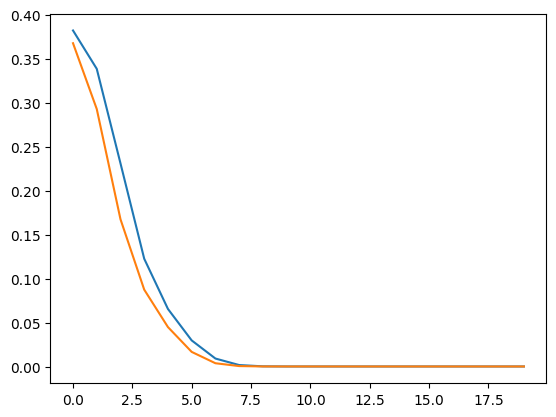
\includegraphics[width=0.73\linewidth]{figures/estimator-loss.png}
\caption{Retained estimator training and validation losses. The two plotted
series should be interpreted alongside held-out trajectory and coordinate checks.}
\end{figure}
\begin{figure}[h!]
\centering
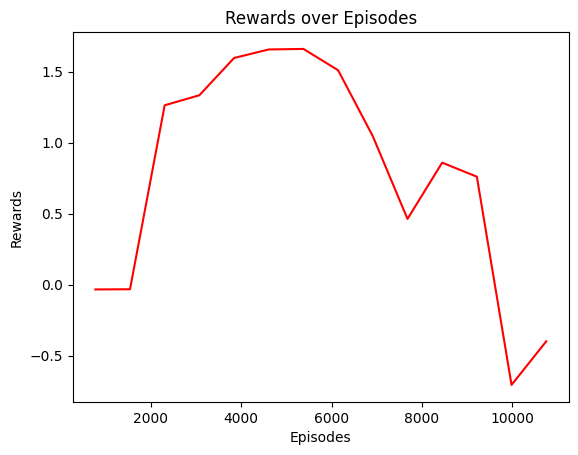
\includegraphics[width=0.47\linewidth]{figures/estimated-state-return.png}\hfill
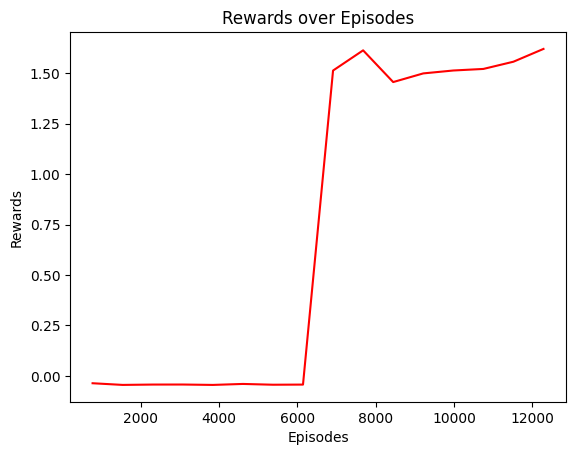
\includegraphics[width=0.47\linewidth]{figures/image-policy-return.png}
\caption{Retained PPO callback evaluations for estimated-state and image
policies. The original horizontal label says ``Episodes'' but records timesteps.}
\end{figure}
The saved end-to-end run has lower recorded return and success than the
state-based expert. This comparison alone cannot separate supervision,
optimization, observation ambiguity, and interaction-budget effects. A useful
new experiment would match evaluation seeds, report uncertainty, and compare
the deployed pipelines on their own observation inputs.

\textbf{Solution scope.} The architecture and tensor shapes follow directly
from the specified layers. The evaluation distinctions identify what the
saved measurements actually tested. The revised wrappers and normalization
settings require fresh runs; historical values do not validate the revised code.
\end{document}
